% IPP
% Projekt - 1.
% Juraj Holub
% xholub40@stud.fit.vutbr.cz

\documentclass[a4paper, 10pt]{article}
\usepackage[utf8]{inputenc}
\usepackage[english]{babel}
\usepackage[T1]{fontenc}
\usepackage[left=2cm,top=2.5cm, right=2cm]{geometry}
\usepackage{hyperref}
\usepackage{graphicx}
\usepackage{float}

\title{Documentation of Project Implementation for IPP 2018/2019 }
\author{Name and surname: Juraj Holub\\ Login: xholub40}
\date{}

\begin{document}
	\maketitle
	\thispagestyle{empty}

% proposal of solution
\section{Proposal of solution} \label{proposal}

    This section introduces the proposed implementation. Figure \ref{obr1} shows the scheme of the implemented interpret. The program starts with parsing source IPPcode19 program in XML representation to program inner representation. In this phase program done all necessary syntactic analyses. In the next step, application execute a parsed sequence of IPPcode19 instructions. In case of any syntactic or semantic error, interpret stop execute source code and return a specific error value. Interpret also generate a brief error message to the standard error stream.

\begin{figure}[H] 
	\centering
	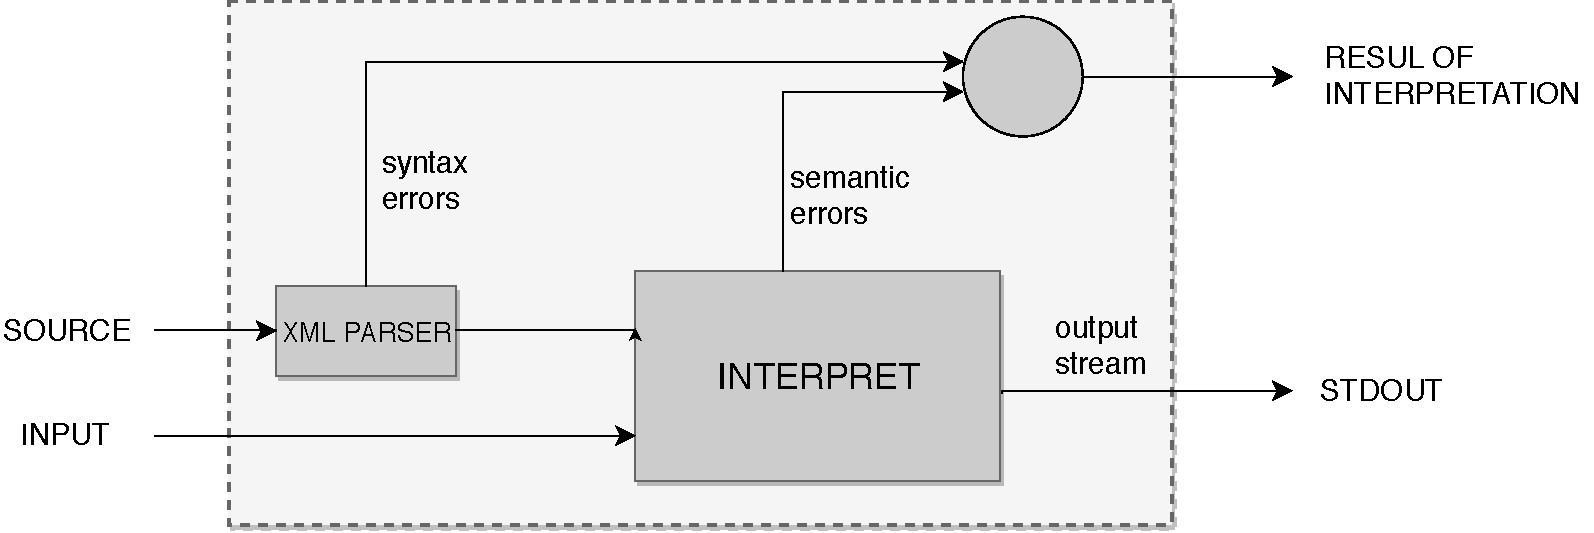
\includegraphics[width=.5 \paperwidth]{interpret.pdf}
	\caption{Scheme of IPPcode19 program interpretation.}
	\label{obr1}
\end{figure} 

\section{Implementation details}
Implementation of the solution proposed in section \ref{proposal} is parted to logical blocks described in this section.
\begin{itemize}
\item \textbf{XML parser}: Class parse raw XML representation of source program to the ordered list of IPPcode19 instructions. Parser class uses python3 library \href{https://docs.python.org/2/library/xml.etree.elementtree.html}{The ElementTree XML API} which provide all necessary syntactic analyses of input XML. Class also verifies syntactic correctness of every instruction (for example XML representation of instruction is correct but IPPcode19 syntactic meaning is incorrect). If any error was found then program finish and interpretation itself never occurs.
\item \textbf{Interpret}: At the beginning, the interpret iterate all instructions and done fast analyse. If analysed instruction is label then interpret saves information about position and name. After this phase program launch interpretation and one by one execute instructions. At this point, if an actually executed command is an instruction of jump then interpret knows about the existence of requested label and his position in the code. For every instruction, there is implemented one method which executes it. Interpret class save data about all variables, their frames, about data stack and call stack. All instruction operands data are converted to python data types. This approach allows transfer responsibility of runtime type conversion and analyses to python interpret. 
\item \textbf{Error handling}: Interpret raises the specific exception in case of any runtime error. Every semantic error is represented by a specific user-defined exception. These exceptions hold data about the actual situation in the program. Interpret inform a user to standard error stream about type of error, data which caused it and position in the code.
\item \textbf{String convertor}: Source programming language allows declaring string literals with escape sequences. String converter class transform input string literal with escape sequences to a human-readable format. The converter is implemented like a finite state machine.
\end{itemize}

\end{document}
